%%!TEX encoding = UTF-8 Unicode

% Several lines in file have comments suggesting common packages for the
% typical thesis in informatics or electronics developed at UA
% uncomment/comment the lines as required for your work
% Before each optional line you will have a small comment

% According to UA rules, font size should range from 10 to 12pt.
\documentclass[11pt,a4paper,openright,twoside,onecolumn]{memoir}

\listfiles
\fixpdflayout

\usepackage[utf8]{inputenc}

% Select Computer Modern Typewritter (For bold ttfamily in listings)
\usepackage{lmodern}
% OR... Bera Mono
%\usepackage[scaled]{beramono} % TTT Font
%\usepackage{anyfontsize} % As the name says...

\usepackage[T1]{fontenc}

% Enable for for Overleaf support
\usepackage{ifthen}
\def\useoverleaf{0}  % change to non-zero (for instance, 1) to enable it

\makeatletter
\newcommand{\makecoverfile}[0]{%
  \immediate\write18{latexmk -pdf cover.tex}%
}
\makeatother

% For PDF merging
\usepackage{pdfpages}

% Set DPI to 300
\pdfpxdimen=\dimexpr 1in/300\relax

% Allow the use of a larger number of packages
\usepackage{morewrites} 

% For English and Portuguese languages
% Portuguese will be the default.
% Uncomment \setlanguage below to change it
\usepackage[english,portuguese]{babel}

% Uncomment to use a custom date format
%\usepackage{datetime}
%\newdateformat{thesisdate}{\monthname[\THEMONTH] \THEYEAR} % Month Year

% Make pdf look better
\usepackage{microtype} 

% Uncomment to enable floats on facing pages
%\usepackage{dpfloat}

% Side by side figures
% Eg. Fig 1a, Fig 1b
\usepackage[hang,small,bf]{caption}
%\let\tion\undefined
%\let\subfloat\undefined
\usepackage{subcaption}

%\RequirePackage{textcase}

% Dropped Caps
%\usepackage{lettrine}

% Configure Hyperlink color
% As a matter or style, you may use this to enable/disable color boxes on links
%\usepackage[breaklinks=true,colorlinks=false,linkcolor=blue]{hyperref}
% Or use the default values provided by the hyperref package
\usepackage[hidelinks]{hyperref}

% Redefine section names according to your preference
%\def\sectionautorefname{Section}
%\def\chapterautorefname{Chapter}
%\def\figureautorefname{Figure}
%\def\listingautorefname{Listing}
%\def\tableautorefname{Table}

% Redefine code boxes
\ifthenelse{\equal{\useoverleaf}{0}}
{\usepackage[outputdir=build]{minted}}
{\usepackage{minted}}%

\addto\captionsportuguese{%
  \renewcommand\listingscaption{Código}
}
\fvset{fontsize=\footnotesize} % Make Code blocks smaller than text
\usepackage{csquotes}

% Add support for PDF Comments
\usepackage{comment}
\ifthenelse{\equal{\useoverleaf}{0}}
{\usepackage{pdfcomment}}{}
\usepackage{bookmark} % New Bookmarks

% For Multiple columns in Glossary
\usepackage{multicol}

% Add support for Math symbols
\usepackage{amsmath}
\usepackage{amssymb}

% Add support for graphics
\usepackage{graphicx}

% Add support for Colors
\usepackage{xcolor}

% Add support for the Euro symbol
\usepackage{eurosym}

% Add support for missingfigure and todo
\usepackage{todonotes}

% Setup bibliography with Biber using IEEE style for proper UTF-8 support
\usepackage[backend=biber, style=ieee, sorting=none, natbib=true, mincitenames=1, maxcitenames=2]{biblatex}
\bibliography{bib/references.bib, bib/rfc.bib, bib/network.bib}

% Use acronyms
\usepackage[printonlyused]{acronym} % For acronyms

% Indenting the first paragraph after section start
\usepackage{indentfirst}

% For fixing listoflistings with memoir
\usepackage{xparse}

% Uncomment the next lines to enable chart support through pgf and tikz
% This may require you to install further packages in your Tex system
%\usepackage[version=0.96]{pgf}
%\usepackage{tikz}

% UML support
%\usepackage{pgf-umlsd}

% Trees, Arrows, Mindmaps and other popular objects
%\usetikzlibrary{arrows,shadows,trees,shapes,decorations,automata,backgrounds,petri,mindmap} % for pgf-umlsd

% Package to master SI units
\usepackage[detect-weight=true, binary-units=true]{siunitx}
% For Electric Circuits
%\sisetup{load-configurations = binary}

% Set Voltage direction accordingly
% Option : oldvoltagedirection,nooldvoltagedirection,RPvoltages,EFvoltages
% More information at: https://mirrors.ibiblio.org/CTAN/graphics/pgf/contrib/circuitikz/doc/circuitikzmanual.pdf
% By default this template is using the Old Voltage Direction
%\usepackage[oldvoltagedirection,american,cuteinductors,smartlabels]{circuitikz}
%\usetikzlibrary{calc}
%\ctikzset{bipoles/thickness=1}
%\ctikzset{bipoles/length=0.8cm}
%\ctikzset{bipoles/diode/height=.375}
%\ctikzset{bipoles/diode/width=.3}
%\ctikzset{tripoles/thyristor/height=.8}
%\ctikzset{tripoles/thyristor/width=1}
%\ctikzset{bipoles/vsourceam/height/.initial=.7}
%\ctikzset{bipoles/vsourceam/width/.initial=.7}
%\tikzstyle{every node}=[font=\small]
%\tikzstyle{every path}=[line width=0.8pt,line cap=round,line join=round]

% For inline TT text (e.g. code snippets)
\usepackage{verbatim}

% Frames around figures and allow force placement
\usepackage{float}

% Configure Float style
%\floatstyle{boxed}
%\restylefloat{table}
%\restylefloat{figure}
%\restylefloat{lstlisting}

% For test purposes you may use the lipsum package to create dummy text
\usepackage{lipsum} % REMOVE

%Keep floats inside section!
\usepackage[section]{placeins}
\let \oldsubsubsection \subsubsection
\renewcommand{\subsubsection}[2][]{
  \FloatBarrier
  \oldsubsubsection#1{#2}
}
\let \oldsubsection \subsection
\renewcommand{\subsection}[2][]{
  \FloatBarrier
  \oldsubsection#1{#2}
}
\let \oldsection \section
\renewcommand{\section}[2][]{
  \FloatBarrier
  \oldsection#1{#2}
}
\let \oldchapter \chapter
\renewcommand{\chapter}[2][]{
  \FloatBarrier
  \oldchapter#1{#2}
}



% Use the built-in division styling
\headstyles{memman}

% Include subsections in the TOC
\settocdepth{subsection}

% Numbering down to subsections as well
\setsecnumdepth{subsection}

% extra index for first lines
\makeindex[lines]

% Margins for University of Aveiro Thesis
\setlrmarginsandblock{3cm}{2.5cm}{*}
\setulmarginsandblock{3cm}{3cm}{*}
\checkandfixthelayout

% Or select your custom spacing to make any ajustment
%\addtolength{\parskip}{0.5\baselineskip}
\linespread{1.5}

\newcommand\mainmatterWithoutReset
{\edef\temppagenumber{\arabic{page}}%
  \mainmatter
  \setcounter{page}{\temppagenumber}%
}


%%%%%%%%%%%%%%%%%%%%%%%%%%%%%%%%%%%%%%%%%%%%%%%%%%
% Document begins here
%%%%%%%%%%%%%%%%%%%%%%%%%%%%%%%%%%%%%%%%%%%%%%%%%%

\begin{document}

% Fix the numbering scheme by having a ghost style for page numbering
\pagenumbering{Alph}

\ifthenelse{\equal{\useoverleaf}{0}}{}{\makecoverfile{}}%
\includepdf[pages=-]{cover.pdf}

% Uncomment to enable English
\selectlanguage{english}


% Front matter

%Custom Chapter style named `thesis`
\makechapterstyle{thesis}{% Based on ell
  \chapterstyle{default}
  \renewcommand*{\chapnumfont}{\normalfont\sffamily}
  \renewcommand*{\chaptitlefont}{\normalfont\Huge\sffamily}
  \settowidth{\chapindent}{\chapnumfont 111}
  \renewcommand*{\chapterheadstart}{\begingroup
    \vspace*{\beforechapskip}%
    \begin{adjustwidth}{}{-\chapindent}%
    \hrulefill
    \smash{\rule{0.4pt}{15mm}}
    \end{adjustwidth}\endgroup}
  \renewcommand*{\printchaptername}{}
  \renewcommand*{\chapternamenum}{}
  \renewcommand*{\printchapternum}{%
    \begin{adjustwidth}{}{-\chapindent}
    \hfill
    \raisebox{10mm}[0pt][0pt]{\fontsize{30}{25}\selectfont\chapnumfont \thechapter}%
                              \hspace*{1em}
    \end{adjustwidth}\vspace*{-3.0\onelineskip}}
  \renewcommand*{\printchaptertitle}[1]{%
    \vskip\onelineskip
    \raggedleft {\chaptitlefont ##1}\par\nobreak\vskip 4\onelineskip}}


% Select chapter style from existing or select custom
%\chapterstyle{thesis} % Others: dowding, demo2, dash, chappell, brotherton, bianchi, ger, madsen, tatcher, veelo,indexes)
% thesis can also be used as defined previously
% Check the memoir documentation for the available themes
% Default is veelo
\chapterstyle{veelo}
\makeoddfoot{plain}{}{\thepage}{} % Added by André Zúquete to fix a page numbering issue on the veelo chapter style


% If you feel adventurous you can also define all aspects of your theme
% Use either this input or the chapterstyle before
% % Rules
\newcommand{\thinRule}{\rule{\textwidth}{0.25pt}}

% Customize heading appearances
% Define styles
\newcommand{\partSize}{\Huge}
\newcommand{\partStyle}{\lsstyle\scshape}
\newcommand{\chapterSize}{\Huge}
\newcommand{\chapterStyle}{\lsstyle\scshape}
\newcommand{\chapterAfter}{}
\newcommand{\sectionSize}{\Large}
\newcommand{\sectionStyle}{\scshape\MakeTextLowercase}
\newcommand{\subsectionSize}{\large}
\newcommand{\subsectionStyle}{\scshape\MakeTextLowercase}
\newcommand{\subsubsectionSize}{\large}
\newcommand{\subsubsectionStyle}{\scshape\MakeTextLowercase}
\newlength{\partNumSizePt}
\setlength{\partNumSizePt}{60pt}
\newlength{\chapterNumSizePt}
\setlength{\chapterNumSizePt}{60pt}
\newcommand{\partNumSize}{%
  \fontsize{\partNumSizePt}{1.2\partNumSizePt}\selectfont%
}
\newcommand{\partNumStyle}{\partChapterNumColor}
\newcommand{\chapterNumSize}{%
  \fontsize{\chapterNumSizePt}{1.2\chapterNumSizePt}\selectfont%
}
\newcommand{\chapterNumStyle}{\partChapterNumColor}

% Customize parts
\renewcommand{\partnamefont}{\partSize\partStyle}
\renewcommand{\partnumfont}{\partNumSize\partNumStyle}
\renewcommand{\printpartname}{}
\renewcommand{\printparttitle}[1]{%
  \normalfont\normalcolor\partnamefont #1
}

% Customize chapters
\makeatletter
\setlength{\beforechapskip}{30pt}
\renewcommand*{\chapterheadstart}{\vspace*{\beforechapskip}}
\setlength{\afterchapskip}{3ex}
\setlength{\midchapskip}{3ex}
\renewcommand*{\chapnamefont}{%
  \Large\flushright\chapterStyle\partChapterNumColor%
}
\renewcommand*{\chapnumfont}{\chapterNumSize\chapterNumStyle}
\renewcommand*{\chaptitlefont}{%
  \normalfont\flushleft\normalcolor\chapterSize\chapterStyle%
}
\renewcommand*{\printchaptername}{%
  \chapnamefont\MakeTextLowercase{\@chapapp}%
}
\renewcommand*{\chapternamenum}{\quad}
\renewcommand*{\printchapternum}{%
%  \chapnumfont\textls[-75]{\classicstylenums{\thechapter}}%
 \chapnumfont\textls[-75]{\thechapter}%

}
\renewcommand*{\printchaptertitle}[1]{%
  \chaptitlefont #1
  \chapterAfter
}
\makeatother
% Customize sections and subsections
\setsecnumformat{\csname my#1\endcsname\quad}
\setsecheadstyle{\sectionSize\sectionStyle}
\newcommand{\mysection}{{\thesection}}
\setlength{\beforesecskip}{3em}


\setsubsecheadstyle{\subsectionSize\subsectionStyle}
\newcommand{\mysubsection}{{\normalfont\subsectionSize\thesubsection}}
\setlength{\beforesubsecskip}{3em}

\setsubsubsecheadstyle{\subsubsectionSize\subsubsectionStyle}
\newcommand{\mysubsubsection}{{\normalfont\subsubsectionSize\thesubsubsection}}
\setlength{\beforesubsubsecskip}{2em}

% Customize "Table of ..." appearance
% Customize headings
\newcommand{\renewPrintXTitle}[1]{%
  \renewcommand{#1}[1]{%
    \printchaptertitle{##1}%
  }%
}
\renewPrintXTitle{\printtoctitle}
\renewPrintXTitle{\printlottitle}
\renewPrintXTitle{\printloftitle}

% Customize ToC headings
\renewcommand{\cftpartfont}{\partChapterNumColor\partStyle}
\renewcommand{\cftchapterfont}{\chapterStyle}
\renewcommand{\cftsectionfont}{}
\renewcommand{\cftsubsectionfont}{}
\renewcommand{\cftfigurefont}{}
\renewcommand{\cfttablefont}{}
\newcommand{\cftlstlistingfont}{}

% Increase number width
\newlength{\cftNumWidthIncrease}
\setlength{\cftNumWidthIncrease}{0.25em}
\addtolength{\cftpartnumwidth}{\cftNumWidthIncrease}
\addtolength{\cftchapternumwidth}{\cftNumWidthIncrease}
\addtolength{\cftsectionindent}{\cftNumWidthIncrease}
\addtolength{\cftsubsectionindent}{\cftNumWidthIncrease}
% No leader dots
%\renewcommand*{\cftpartdotsep}{\cftnodots}
%\renewcommand*{\cftchapterdotsep}{\cftnodots}
%\renewcommand*{\cftsectiondotsep}{\cftnodots}
%\renewcommand*{\cftsubsectiondotsep}{\cftnodots}
%\renewcommand*{\cftfiguredotsep}{\cftnodots}
%\renewcommand*{\cfttabledotsep}{\cftnodots}
%\newcommand*{\cftlstlistingdotsep}{\cftnodots}
% Set page numbers immediately after entry text
\newcommand{\tocEntryPageSep}{\hspace{1em}}
\renewcommand{\cftpartleader}{\cftdotfill{\cftdotsep}}
%\renewcommand{\cftpartafterpnum}{\cftparfillskip}
%\renewcommand{\cftchapterleader}{\tocEntryPageSep}
\renewcommand{\cftchapterleader}{\cftdotfill{\cftdotsep}}
%\renewcommand{\cftchapterafterpnum}{\cftparfillskip}
\renewcommand{\cftsectionleader}{\cftdotfill{\cftdotsep}}
%\renewcommand{\cftsectionafterpnum}{\cftparfillskip}
\renewcommand{\cftsubsectionleader}{\cftdotfill{\cftdotsep}}
%\renewcommand{\cftsubsectionafterpnum}{\cftparfillskip}
\renewcommand{\cftfigureleader}{\cftdotfill{\cftdotsep}}
%\renewcommand{\cftfigureafterpnum}{\cftparfillskip}
\renewcommand{\cfttableleader}{\cftdotfill{\cftdotsep}}
%\renewcommand{\cfttableafterpnum}{\cftparfillskip}
\newcommand{\cftlstlistingleader}{\cftdotfill{\cftdotsep}}
%\newcommand{\cftlstlistingafterpnum}{\cftparfillskip}
% Customize page numbers
\newcommand{\tocPageStyle}{\tocPageColor}
\renewcommand{\cftpartpagefont}{\tocPageStyle}
\renewcommand{\cftchapterpagefont}{\tocPageStyle}
\renewcommand{\cftsectionpagefont}{\tocPageStyle}
\renewcommand{\cftsubsectionpagefont}{\tocPageStyle}
\renewcommand{\cftfigurepagefont}{\tocPageStyle}
\renewcommand{\cfttablepagefont}{\tocPageStyle}
\newcommand{\cftlstlistingpagefont}{\tocPageStyle}

% Abstract
% Remove indents around abstract text
\setlength{\absleftindent}{0pt}
\setlength{\absrightindent}{0pt}
% Change font size to conform with the rest of the document text
\renewcommand{\abstracttextfont}{\normalsize}

% Customize headers and footers including page numbers
\newcommand{\hfTextSize}{\footnotesize}
\newcommand{\headTextStyle}{\lsstyle\scshape\MakeTextLowercase}
\nouppercaseheads
\makeevenhead{headings}%
             {\hfTextSize\thepage}%
             {}%
             {\hfTextSize\headTextStyle\leftmark}
\makeevenhead{plain}%
             {\hfTextSize\thepage}%
             {}%
             {\hfTextSize\headTextStyle\leftmark}
\makeoddhead{headings}%
            {\hfTextSize\headTextStyle\rightmark}%
            {}%
            {\hfTextSize\thepage}
\makeoddhead{plain}%
            {\hfTextSize\headTextStyle\rightmark}%
            {}%
            {\hfTextSize\thepage}


% Customize captions
\newcommand{\captionSize}{\small}
\newcommand{\captionStyle}{\scshape}
\newcommand{\captionWidthRatio}{0.9}

\captionnamefont{\captionSize\captionStyle}
\captiontitlefont{\captionSize}
\captiondelim{ -- }
\captiontitlefinal{}
\changecaptionwidth
%\captionwidth{\captionWidthRatio\textwidth}

% Define colors
%\newcommand{\titleColor}{\color[rgb]{0.616, 0.0627, 0.176}}
\newcommand{\titleColor}{\color[rgb]{0,0,0}}

\newcommand{\partChapterNumColor}{\titleColor}
\newcommand{\dropCapColor}{\titleColor}
%\newcommand{\tocPageColor}{\color[rgb]{0.0980, 0.329, 0.651}}

\newcommand{\tocPageColor}{\color[rgb]{0, 0,0}}
\definecolor{shade0}{rgb}{1.0 , 1.0 , 1.0 }
\definecolor{shade1}{rgb}{0.9 , 0.9 , 0.9 }
\definecolor{shade2}{rgb}{0.8 , 0.8 , 0.8 }
\definecolor{shade3}{rgb}{0.65, 0.65, 0.65}
\definecolor{shade4}{rgb}{0.45, 0.45, 0.45}
\definecolor{shade5}{rgb}{0.0 , 0.0 , 0.0 }



%Exclude sub figures from List of Figures
%\captionsetup[subfloat]{list=no}

% Texts
\newenvironment{introduction}
{%
  \begin{minipage}{\textwidth}%
   \itshape%
}
{%
  \end{minipage}%
  \par\addvspace{2\baselineskip plus 0.2\baselineskip minus 0.2\baselineskip}%
}

% Select Page style
\pagestyle{plain}


\frontmatter

\tightlists
\midsloppy
\raggedbottom

\setcounter{tocdepth}{2} %subsections are added to the TOC
\setcounter{secnumdepth}{4} %subsubsections are numbered

% Initial document tables start here: TOC, LOF, LOT, Glossary
% Table of contents with slightly smaller font
\cleardoublepage
{\small\tableofcontents}

% List of figures with slightly smaller font
\cleardoublepage
{\small\listoffigures}

% List of tables with slightly smaller font
\cleardoublepage
{\small\listoftables}

% List of code snippets

% Fix for Listings with memoir

\RenewDocumentCommand \chapter { s O{#3} m }{%
  \FloatBarrier
  \IfValueTF{#1}  % if optional star is seen
    {\oldchapter*{#2}}
    {\oldchapter#1{#2}}
}

\renewcommand{\listingscaption}{Código}
\renewcommand{\listoflistingscaption}{Lista de Excertos de Código}
\cleardoublepage
{\small\listoflistings}
\addcontentsline{toc}{chapter}{\listoflistingscaption}

% Reset Chapters
\renewcommand{\chapter}[2][]{
  \FloatBarrier
  \oldchapter#1{#2}
}

% Print Glossary
{\small\chapter{Glossário}

\footnotesize
\SingleSpacing

\begin{multicols}{2}
\begin{acronym}[AAAAAA]

	\acro{ict}[ICT]{Information and Communication Technology}
	\acro{isp}[ISP]{Internet Service Provider}
	\acro{dsl}[DSL]{Digital Subscriber Line}
	\acro{adsl}[ADSL]{Asymmetric Digital Subscriber Line}
	\acro{docsis}[DOCSIS]{Data Over Cable Service Interface Specification}
	\acro{epon}[EPON]{Ethernet Passive Optical Network}
	\acro{wdm}[WDM]{Wavelength Division Multiplexing}
	\acro{oxc}[OXC]{Optical Cross-Connect}
	\acro{tcp}[TCP]{Transmission Control Protocol}
	\acro{ip}[IP]{Internet Protocol}
	\acro{cpe}[CPE]{Customer Premises Equipment}
	\acro{watt}[W]{Watt}
	\acro{kilowatt-hour}[kWh]{Kilowatt-hour}
	\acro{gigabyte}[GB]{Gigabyte}
	\acro{lan}[LAN]{Local Area Network}
	\acro{wan}[WAN]{Wide Area Network}
	\acro{wpan}[WPAN]{Wireless Personal Area Network}
	\acro{wlan}[WLAN]{Wireless Local Area Network}
	\acro{wman}[WMAN]{Wireless Metropolitan Area Network}
	\acro{wwan}[WWAN]{Wireless Wide Area Network}

\end{acronym}
\end{multicols}

}

%%%%%%%%%%%%%%%%%%%%%%%%%%%%%%%%%%%%%%%%%%%%%%%%%%%%%%%
% Main document starts here
%%%%%%%%%%%%%%%%%%%%%%%%%%%%%%%%%%%%%%%%%%%%%%%%%%%%%%%

\mainmatter

% Line spacing: 1.5 pt 
\OnehalfSpacing

%%%%%%%%%%%%%%%%%%%%%%%%%%%%%%%%%%%%%%%%%%%%%%%%%%%%%%%
% Start of Thesis text 
%%%%%%%%%%%%%%%%%%%%%%%%%%%%%%%%%%%%%%%%%%%%%%%%%%%%%%%

% Uncomment to add further chapters
%

\chapter{Introdução}
\label{chapter:introduction}

\begin{introduction}
A short description of the chapter.

A memorable quote can also be used.
\end{introduction}



\section{Acrónimos}

Primeira e seguintes referências: \ac{h2o}, \ac{h2o}

Plural, acrónimo expandido e curto: \acp{h2o}, \acs{h2o}, \acl{h2o}

Com citação\footnote{Necessária entrada na bibliografia}: \ac{adsl}, \ac{adsl}


\section{Fontes}

\begin{itemize}
\item{\tiny Tiny}
\item{\scriptsize Scriptsize}
\item{\footnotesize Footnotes}
\item{\small Small}
\item{\normalsize Normal}
\item{\large large}
\item{\Large Large}
\item{\LARGE LARGE}
\item{\huge huge}
\item{\Huge Huge}
\end{itemize}

\section{Unidades}

Utilizando o pacote \verb|siunitx| é possível utilizar unidades do Sistema Internacional. Exemplo: a aceleração da gravidade é de \SI{9.8}{\metre\per\second\squared} e um ficheiro ocupa \SI{1}{\mebi\byte}. 

\section{Code Blocks}
%\lipsum[5]
Uma listagem pode ser apresentada com o ambiente \texttt{listing}, que é um float (objeto flutuante, tal como uma figura ou uma tabela).

A listagem em Código~\ref{lbl:snippet-test} mostra um exemplo em C.

\begin{listing}[h]
\begin{minted}{c}

#include <stdio.h>
#define N 10
/* Block
 * comment */
 
int main()
{
    int i;
 
    // Line comment.
    puts("Hello world!");
 
    for (i = 0; i < N; i++)
    {
        puts("LaTeX is also great for programmers!");
    }
 
    return 0;
}
\end{minted}
\caption{This caption appears below the code.}
\label{lbl:snippet-test}
\end{listing}

%\lipsum[5]

\section{Citações}

Algumas formas distintas de citar:

\begin{itemize}
    \item \textbf{Apenas referência}:~\cite{rfc44}
    \item \textbf{Apenas data}:~\citedate{rfc44}
    \item \textbf{Apenas ano}:~\citeyear{rfc44}
    \item \textbf{Apenas autor}:~\citeauthor{rfc44}
    \item \textbf{Apenas editor}:\citelist{rfc44}{organization}
    \item \textbf{Autor e referência}:\citet{rfc44}
\end{itemize}



\chapter{Introduction}
\label{chapter:introduction}

\begin{introduction}

Energy consumption has been a topic of discussion lately due to the increase of global warming. The \ac{ict} sector is responsible for around 4-6\% of the global eletricity use in 2020 \citet{UK-parliament}. The main contributer to the energy consumption of the \ac{ict} sector are datacenters, which account for XXX\% (\citet{check source}). With the increase of internet use and the need to process large amounts of data, the energy consumption of the \ac{ict} sector will only increase further.

The primary objective of this thesis is to analyse data compression algorithms and their impact on the energy consumption of the \ac{ict} sector.
To achieve this objective, a model of the energy consumption of the \ac{ict} sector was develop, along side a web calculator to compare different compression algorithms on several uses cases. 

In this chapter, we will present reasearch questions, followed by the hypotheses and objectives of the thesis. We will then present the risk assessment and impact of the thesis, concluding with the contributions of the thesis. 

\end{introduction}

\section{Researh questions}

To define the scope of the thesis, the following research questions were defined:

- What is the system boundary of the model?

- How to test the accuracy of the model?

- What is the impact of each component of the model?

\section{Hypotheses}

\section{Objectives}

- Study the current energy models of the internet

- Develop an aggregated model.

- Develop a web calculator to show the model

- Create case studies to benchmark the model


\section{Risk assessment and impact}

\section{Contributions}

\section{Thesis structure}

This thesis is divided into 6 chapters. After this introduction (chapter 1), a background on the concepts covered, such as network structure and compressions, is presented in chapter 2. Chapter 3 focuses on the recent works that have modeled part of the internet. An aggregation of these recent models will be presented in chapter 4. Chapter 5 will present the web calculator developed to show the model, along side with use cases on how to use the web calculator. Finally, chapter 6 will present the conclusions of the thesis and future work.


% - chapter 1: introduction
% - chapter 2: background
% - chapter 3: related work
% - chapter 4: Energy model
% - chapter 5: web calculator and use cases
% - chapter 7: conclusion


\chapter{Background}
\label{chapter:background}

\begin{introduction}
    
    The modelling of the energy consumption of the \ac{ict} sector is a complex task, because it involves modelling several systems, each with their distinct topologies and external factors.

    In this chapter we can find a description of the topology of the different systems that comprise the \ac{ict} sector and a highlight on the main component of each system. Moreover, the chapter also includes a description on the basics of compression algorithms and the different types of compression algorithms.

\end{introduction}

\section{System Boundaries}
\label{section:system_boundaries}

The definition of system boundaries is an important factor in the modelling of energy consumption. As seen in the compilation of studies made by \citet{Aslan2018}, the system boundaries are one of the main factors for the discrepancies of the results.

The common consensus is that the system boundaries for the model of the internet should exclude datacenters and user devices, as shown by \citet{Coroama2014}. Our study however won't be modeling only the internet but also the impact on datacenters and of the compression/decompression algorithm in the end user device. So the overall system boundary will include all the \ac{ict} sector. 

So our study divides the system boundary in three main components: the network, datacenters and the end user devices (Figure \ref{figure:system_boundaries}). The network is divided in three main components: \ac{cpe}, Access Network and Core Network. The datacenter is also divided in three components: Servers, Storage and Datacenter Network. Lastly the end user devices only includes the compression/decompression algorithm cost. 

\begin{figure}[h]
    \centering
    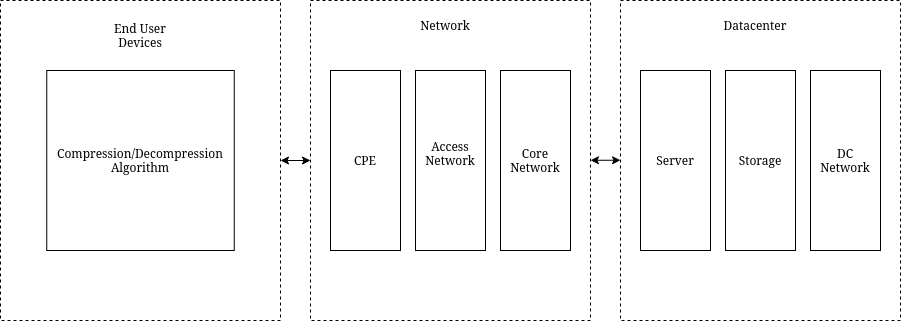
\includegraphics[width=1\textwidth]{figs/System_Boundary.png}
    \caption{Complete system boundary of the model and subsystem of each component.}
    \label{figure:system_boundaries}
\end{figure}

\section{Internet}

The internet is the most complex component of the model.
Internet started has an interconnection of a small number of local university networks, which were composed of a few routers and cables. Nowadays, the internet is a global network of networks, composed of millions of routers, switches and cables, that interconnects billions of end users. This communication is made possible by the use of the \ac{tcp} and \ac{ip} protocols.

Because of its complexity the system is usually divided into smaller components. However, the delimitation on where each component begins and ends can vary from paper to paper. In this thesis, we use the delimitation proposed by \citet{Coroama2015} and \citet{Schien2015}, which divides the internet in four main components: \ac{cpe}, access network, \ac{ip} core network and undersea cables.

\subsection{\acl{cpe} and Access Network}

There are several technologies used to connect the user to the Ethernet. They can be either wired or wireless and can be part of the \ac{cpe} layer or access network layer. Figure \ref{figure:network_technologies} highlights which technologies are currently used and in what layer they belong to.

\begin{figure}[h]
    \centering
    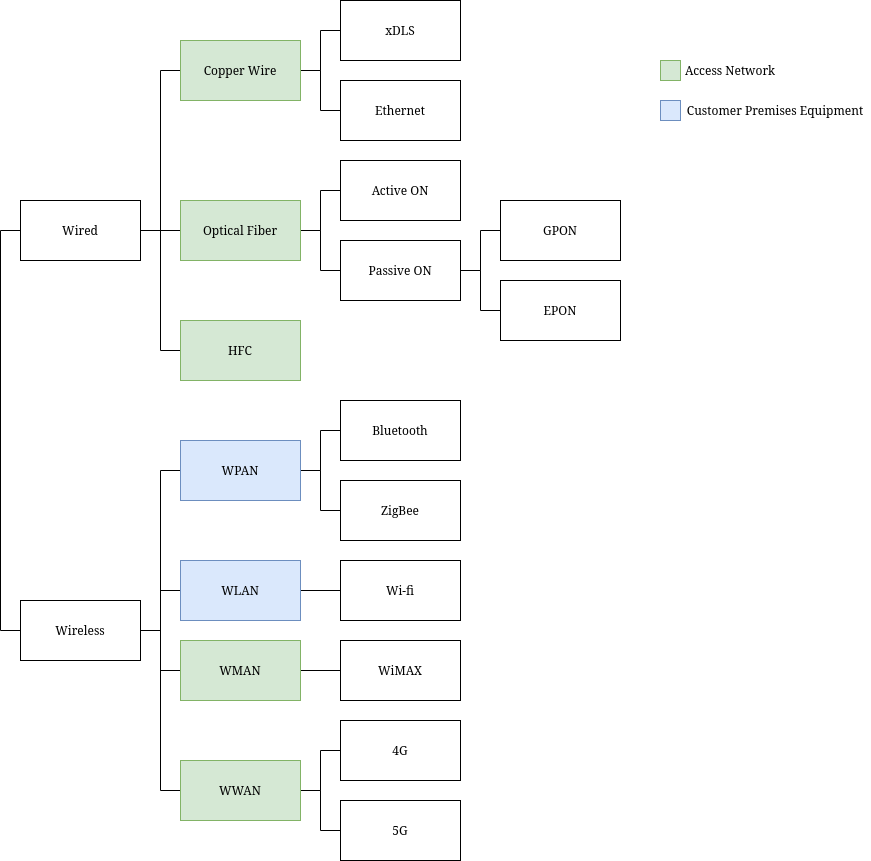
\includegraphics[width=0.8\textwidth]{figs/network_technologies.png}
    \caption[Network technologies used in Access Networks and CPE]{Network technologies used in Access Networks and CPE. In green are the technologies used in the access network and in blue are the technologies used in the CPE. Adapted from \citet{forum:huawei}.}
    \label{figure:network_technologies}
\end{figure}

The first layer and most simple one is the \ac{cpe}. The \ac{cpe} is the equipment that is installed in the end user premises. 
The equipment is usually provided by the \ac{isp} and normally consists of a gateway that acts as a modem and a router.
A modem is used to convert the signal from the \ac{isp} to a signal that can be used by the router. The router is used to connect the end user devices to the internet. The user can connect to the routers either by cable or by wireless technology like Wi-Fi. 

Access networks serve as the connection between the \ac{cpe} and the core network. All users are connected to a central office where traffic is aggregated and then transferred to the core network.
The access network incorporates any technology that establishes the connection between the end user and the \ac{isp} and this technology it is not own by the user. % So a user can connect to the internet by either a modem or a cellular tower but only the cellular tower is part of the access network. 

Traffic in the access network is highly variable. The equipment used in the access network has a power consumption that is largely constant in time and thus load-independent \cite{Vereecken2011}.

\subsubsection{Access Network Wired technologies}

The most popular wired connections are \ac{dsl}, coaxial cable and fiber-optics.

\begin{itemize}

    \item \ac{dsl} provides internet access over existing analog telephone lines. So, existing telephone service providers offer \ac{dsl} service. With this technology, user voice and data traffic go through the analog lines. \ac{dsl} uses high frequencies for data transmission and with the help of \ac{dsl} filter data traffic do not interference with voice traffic.
    There are different DSL types. Currently, \ac{adsl} is the most used \ac{dsl} type in the world. 

    \item \ac{hfc} uses the same coaxial cable that is used for cable television. It uses the \ac{docsis} standard to provide internet access.

    \item Fiber-optic networks use light pulses transmitted through glass or plastic fibers, which produce high bandwidth and transmit speeds. 
    The fibers are also more resistant to interference and signal degradation, making them better suited for sending data over long distances without losing signal quality.
    Fiber optics technology, namely \ac{epon}, have become the most popular choice for wired access network technology. \ac{epon} is a point-to-multipoint network, which means that a single optical fiber is used to serve multiple end users. This is done by using a passive optical splitter, which splits the signal into multiple data streams that are sent to each end user.

\end{itemize}


\subsubsection{Access Network Wireless technologies}

Wireless access networks use radio waves to provide fixed or mobile access services for users. 
According to coverage range classification, the broadband wireless access technology are generally divided into different categories, such as: \ac{wpan}, \ac{wlan}, \ac{wman}, and \ac{wwan}. However, only technologies in the \ac{wman} and \ac{wwan} fall into the umbrella of what we refer to as the access network.

The area coverage of \ac{wman} is in the order of kilometers and there are two prominent technologies to establish internet access, \ac{lmds} and \ac{wimax}.

\begin{itemize}

    \item \ac{lmds} is a multipoint communication system. It is used to provided network connectivity to buildings. These are great technologies for last mile connectivity, because they are more cost-effective than wired technologies and can be deployed faster than fiber \cite{forum:imda}.

    \item \ac{wimax}  is based on IEEE 802.16. It provides fixed, mobile or portable wireless connections, with high speeds that can reach up to 70 \ac{mbps} \cite{forum:ctrfantennasinc}.

\end{itemize}

The \ac{wwan} has a bigger range that the \ac{wman} and is used to provide internet access to mobile devices.
\ac{wwan} uses telecommunication cellular network technologies such as 2G, 3G, 4G LTE, and 5G to transfer data.


\subsection{Core Network}

Core networks consist of several core nodes that are interconnected by \ac{wdm} optical fiber links.

\ac{wdm} is a fiber-optic transmission technique that enables the use of multiple light wavelengths (or colors) to send data over the same medium. Two or more colors of light can travel on one fiber, and several signals can be transmitted in an optical waveguide at differing wavelengths or frequencies on the optical spectrum. 

Each core node is composed by a mix of several layers of technologies stacked on top of each other. Typically, it is composed of a \ac{ip} layer, a \ac{wdm} layer and a \ac{oxc} layer.

From a broad perspective, core nodes operate on an optical-electrical-optical basis. This implies that any optical traffic undergoes conversion into the electronic domain and is then processed by the node, regardless of whether the traffic is terminated at that node. Typically, a node comprises several \ac{wdm} transmit and receive cards, commonly known as transponders or transceivers, which are linked to an \ac{ip} router. The \ac{ip} router, in turn, can establish connections with various access routers.

\section{Datacenters}

Datacenters are facilities that house numerous computing and storage devices. They provide users with the opportunity to host their applications as well as store data. Their use is widespread, and their energy impact is substantial, as they are responsible for  1-1.3\% of the global energy consumption \cite{IEA}.

Datacenters are composed of electronic equipment for communication, data processing and storage. The quantity and type of equipment depends on the type of datacenter. Usually, we can distinguish the type of datacenter by its size and processing power. \citet{Shehabi2016} classifies datacenters in the following categories:

\begin{itemize}
    \item Closet;
    \item Room;
    \item Localized;
    \item Midtier;
    \item High-end;
    \item Hyperscale.
\end{itemize}

The main contributors for the energy consumption of datacenters are the servers, the network and the storage devices. Each type of datacenter has a different efficiency in the use of energy. The efficiency of a datacenter is measured by the \ac{pue}, which is the ratio between the total energy consumption of the facility and the energy consumption of the \ac{it} equipment. The closer it is to one, the better the efficiency of the datacenter.

\subsection{Datacenter Servers}

Datacenter servers are the main component of the datacenter. The servers are computers with the resources capable of executing applications and processing data.

As the main component of the datacenter, they are also the main contributor for the energy consumption of it. According to \citet{Cheung2018} and \citet{Dayarathna2016} the servers account for around 70\% of the energy consumption of the datacenter, ignoring cooling and other non \ac{it} factors.


\subsection{Datacenter Storage}

Storage in datacenters is composed of several \acp{hdd} and \acp{ssd} that are connected to the servers. The storage configuration can be divided in three categories: \ac{das}, \ac{nas} and \ac{san} \cite{Storage101}.

\subsubsection{\acl{das}}

As the name suggests, the storage devices connect directly to the server without any networking. \ac{das} can connect either internally or externally, as a single drive or an array of \ac{raid}. 

Of the three types, \ac{das} is the easier and cheapest option. However, it is also the least scalable and the least flexible, because the server has a limited number of ports and expansion slots.

\subsubsection{\acl{nas}}

\ac{nas} is a centralized file-level storage system, that is connected to the server via the network. \ac{nas} is composed of a storage device with an \ac{os} that is optimized for file storage and sharing.

It includes built-in fault tolerance, management capabilities, and security protections, and it can support features such as replication and data deduplication.

\subsubsection{\acl{san}}

\ac{san} is a decentralized block-level storage system, that is connected to the server via the network. It presents a pool of block-level storage to the server, which the server can then format and partition as it sees fit.

It is composed of storage arrays (\acp{raid}), servers for managing data access, storage management software, \acp{hba}, and any physical components that make up the network's infrastructure.

\subsection{Datacenter Network}

Typically, datacenter networks are composed of switches, routers and other hardware components that provide the connectivity and security to run applications and process data on the servers. 
According to \citet{Cheung2018} and \citet{Dayarathna2016} the network accounts for around 10\% of the energy consumption of the datacenter. 

Today there are three main topologies that datacenters can follow, but larger datacenters can use two or all three of them. Each topology has its own advantages and disadvantages, and the choice of topology depends on the type of datacenter and the type of applications that it will be hosted \cite{commScope}.

\subsubsection{Centralized}

This model is more used by smaller datacenters. There are separated environments for the server and storage, with dedicated  cables that connect the storage server cabinets to the storage.  

\subsubsection{\ac{eor}}

This topology consists in distributing network resources, as seen in Figure \ref{figure:eor_topology}. The servers are placed in rows and the network resources are placed at the end of each row. This solution is recommended by the  ANSI/TIA-942 Data Center Standards \cite{ANSI/TIA-942} and is very scalable, repeatable, and predictable.

\begin{figure}[h]
    \centering
    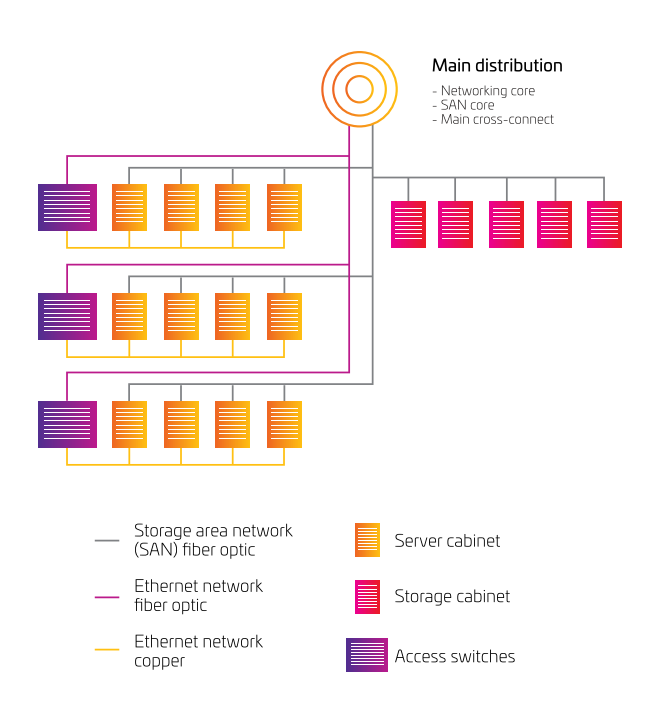
\includegraphics[width=0.8\textwidth]{figs/eor_topology.png}
    \caption[End of Row topology.] {End of Row topology, adapted from \citet{commScope}.}
    \label{figure:eor_topology}
\end{figure}

\subsubsection{\ac{tor}} 

Top of the rack consists on two or more switches on top of each server cabinet, as shown in Figure \ref{figure:tor_topology}. It is cost-effective, because it reduces the number of copper cables between racks. The rack is linked to the data center network by an Ethernet switch, often through a fiber cable. This fiber cable is a direct link from the common aggregation area to the rack.
In the \ac{tor} approach, every rack in the data center network is a separate entity that eases its management. Any change, upgrade, or malfunction in the rack usually affects that rack only.

\begin{figure}[h]
    \centering
    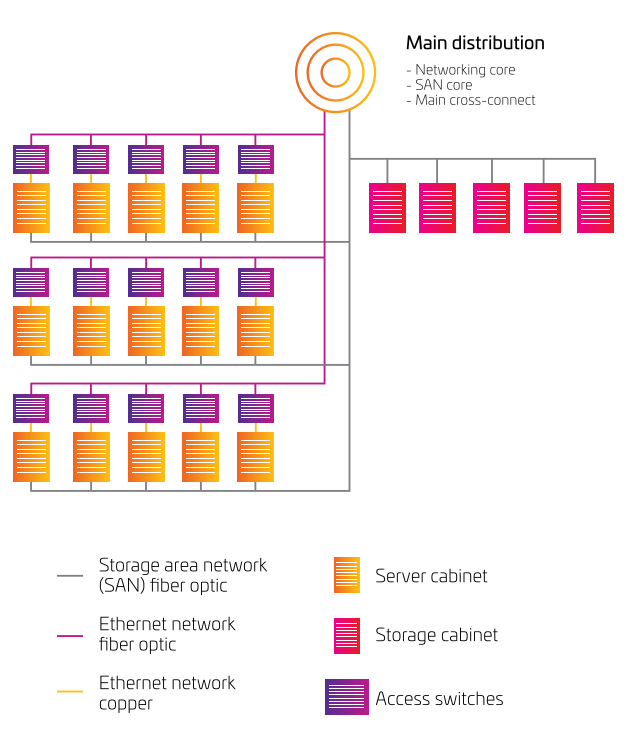
\includegraphics[width=0.8\textwidth]{figs/tor_topology.png}
    \caption[Top of Rack topology.] {Top of Rack topology, adapted from \citet{commScope}.}
    \label{figure:tor_topology}
\end{figure}

\section{Data compression algorithms}

Compression algorithms are used to reduce the size of a file or data stream. They have been used in applications where the cost of storage or transmission is high.

With the increase of the use of the internet and the increase of the amount of data that are stored and transmitted, compression algorithms have become a standard in the \ac{ict} sector.

\subsubsection{Lossless compression}

Lossless algorithms usually exploit the redundancy present in data to reduce the size without losing any information. Among the lossless algorithms, the Lemple-Ziv (LZ) family of algorithms are the most popular. One popular image format that uses lossless compression is the \ac{png} format. The \ac{png} format uses the DEFLATE algorithm \cite{rfc1951}, which is a combination of LZ77 and Huffman coding.

\subsubsection{Lossy compression}

Lossy compression algorithms are used when the loss of information is acceptable. They are usually used in multimedia applications, where the loss of information is not noticeable, or is tolerable by the end user.

\subsection{Compression algorithms overview}
\label{section:compression_algorithms_overview}

Compression algorithms can be divided in two categories based on the type of data that they are used to compressing. General purpose algorithms can be used to compress any type of data. Specific algorithms, on the other hand, are developed to compress a specific type of data, like images, audio or even genetic data, and are usually more efficient in their data type than general purpose algorithms.

There exists several compression algorithms available, their characteristics are summarized in Table \ref{table:compression_algorithms}.

\begin{table}
\caption{Compression algorithms and their characteristics.}
\label{table:compression_algorithms}
\begin{center}
    \begin{tabular}{|| c | c | c ||}
        \hline
        Name & Data type & Reference \\
        \hline
        Gzip        & Any & \citet{rfc1952}\\ \hline
        Zstandard   & Any & \citet{rfc8878}\\ \hline
        Bzip2       & Any & \citet{bzip2}\\ \hline
        LZMA        & Any & \citet{lzma}\\ \hline
        Cmix        & Any & \citet{cmix}\\ \hline
        PAQ1        & Any & \citet{Mahoney2002}\\ \hline
        NNCP        & Any & \citet{NNCP}\\ \hline
        MFCompress  & FASTA, multi-FASTA & \citet{Pinho2014}\\ \hline
        Jarvis3     & FASTA, FASTQ & \citet{jarvis3}\\ \hline
        Naf         & FASTA, FASTQ & \citet{Kryukov2019}\\ \hline
        Leon        & FASTA, FASTQ & \citet{Benoit2015}\\ \hline
        Agc         & FASTA & \citet{Deorowicz2023}\\ \hline
        Fqzcomp     & FASTQ & \citet{fqzcomp}\\ \hline
        Quip        & SAM/BAM & \citet{Jones2012}\\ \hline
    \end{tabular}
\end{center}
\end{table}

\subsubsection{General purpose algorithms}

As stated above, compression algorithms can be divided into two categories, general purpose and specific algorithms. In terms of general purpose algorithms, we have the most popular algorithms, Zstandard, Gzip, Bzip2 and LZMA \cite{GeekyHumans}.

Zstandard and Gzip are both lossless compression algorithms based on the DEFLATE algorithm, which uses a combination of both LZ77 and Huffman coding. Zstandard is the most recent algorithm and was developed by Facebook, offering a much faster compression and decompression than its predecessors. Gzip was created as an alternative to the compress program in Unix systems, because of the Unisys and IBM patents covering the LZW algorithm.

Bzip2 is a lossless compression algorithm based on the Burrows-Wheeler transform. It is more efficient than DEFLATE but is also slower. Even though it can be used in any type of data it is most efficient in text based data. The algorithm is composed of several compression techniques such as \ac{rle}, Burrows-Wheeler transform, move-to-front transform and Huffman coding.

LZMA is a lossless compression algorithm based on the Lempel-Ziv-Markov chain algorithm. It is used by the 7zip file archiver and the xz file format.

Cmix and PAQ are both context mixing compression algorithms. They use more than one model to predict the next symbol in a sequence, it usually results in a more accurate prediction than using only one model. Cmix uses several machine learning models, while PAQ1, a version of the PAQ, uses a weighted average of 5 bit-level predictors.

NNCP also uses machine learning models, in this case it uses pure neural network models based on the \ac{lstm} and Transform model.

\subsubsection{Specific algorithms}

In terms of specific algorithms, we focus on algorithms that compress genome sequences. These algorithms compress files that are in the FASTA, FASTQ and \ac{sam}/\ac{bam} formats.

\subsubsection{Genome sequence formats}

Genome sequencing is a process that determines the order of the nucleotides in a genome, it turns sequences of genomes into data that can be stored and analyzed. The genome sequence is usually stored in a file, which can be in several formats. The most common formats are FASTQ, FASTA, \ac{sam}/\ac{bam} and \ac{vcf}.

FASTQ is a text-based format that stores the biological sequence and its corresponding quality scores. Each entry of the file is composed of 4 lines. The first line is the sequence identifier, the second line is the genetic sequence (the nucleotide bases A, C, T, G and N), the third line is a separator, lastly the fourth line is the quality score of each base.

FASTA is also a text-based format that stores the biological sequence. However, it only stores the headers and nucleotide bases sequenced, which makes it more compact than FASTQ.

\ac{sam}/\ac{bam} are the text and binary versions of the same format. They are used to store the alignment of the sequenced reads to a reference genome. The file is composed of a header and a body. The header contains information about the reference genome and the body contains the alignment of the reads. They reduce the space needed to store a genetic sequence however they are dependent on a reference genome.

Lastly \ac{vcf} is the standard file format for storing variation data. It is used by large scale variant mapping projects such as IGSR. It is also the standard output of variant calling software such as GATK and the standard input for variant analysis tools such as the VEP or for variation archives like EVA.
VCF is a preferred format because it is unambiguous, scalable and flexible, allowing extra information to be added to the info field. Many millions of variants can be stored in a single VCF file. 

MFCompress was designed and implemented in \ac{ieeta}. It is a tool for compressing FASTA and multi-FASTA files, achieving compression gains of almost 50\%. The algorithm bases on probabilistic models that comply with the Markov property, i.e. that estimate the probability of the next symbol of the information source using the $k>0$ immediate past symbols (order-k context) to select the probability distribution. 

Jarvis3, NAF and Leon, are tools that compress FASTA and FASTQ files, but all focus on different techniques. Jarvis3 uses neural network models, while NAF is based on the Zstandard algorithm. Leon uses probabilistic models based on "De Bruijin Graph", it has the advantage of not needing to have a reference genome for the execution of the algorithm.

Agc uses a reference genome to compress FASTA files, and in small sequences it uses Zstandard.

Fqzcomp compresses FASTQ files and uses ZPAQ, an algorithm of the PAQ family, to achieve higher levels of compression.

Lastly Quip compresses FASTQ and \ac{sam}/\ac{bam} files using reference-based arithmetic encoding.


% estado da arte de algoritmos especificos
% algoritmos usados pelo ENA european nucleotide archive e SRA
% zstandard gzip bzip2 lzma 
% especificos fqzcomp quip leon 
% dsrc2 

% tipos de dados:
% fastq fasta sum/bam vcf

% seqSqueeze

% mfcompress
% jarvis3
% naf agc

% cmix
% paq1-9
% nncp




\chapter{Related Works}
\label{chapter:related_works}

\begin{introduction}
    Many authors have tackled the problem of estimating the energy consumption of parts of the \ac{ict}. However, very few have tried to estimate the energy consumption of the \ac{ict} as a whole. To make sure that the most appropriate models are used in this thesis, a review of the most recent studies was made. This review includes the criteria for selecting these models, a description on how the models work and the system boundary they act upon, and the pitfalls and assumptions of each model.
\end{introduction}

\section{Systematic review methodology}

The search methodology focused on studies that analyze energy or carbon consumption of parts of the \ac{ict} sector, such as datacenters. The search was based primarily on English language publications, using bibliographic databases such as IEEE Xplore Digital Library (\textbf{link}), ResearchGate (\textbf{link}). ACM Digital Library (\textbf{link}) and Google Scholar (\textbf{link}). Also, to complement the search we used ConnectedPapers (\textbf{link}), a tool that uses the references of a paper to create a graph of papers similar to the reference.

The search was based on primarily done by using a keyword related to the specific area of the \ac{ict} sector in study followed by a keyword related to energy consumption. For example a search for datacenters would be done by using the keywords \textit{"datacenter"} and \textit{"power consumption"}. The search filtered articles to include only those above January 2000. 
From the results gathered papers that showed bottom-up models were privileged over top-down models. 

\section{Energy consumption studies}

In this section, we will present the most relevant studies gathered by the methodology described in the previous section. Each study tackles a different subsystem, however, their boundary delimitation can overlap with others, so we will frame the boundaries of the studies into the system boundaries that we have defined in \ref{section:system_boundaries}.

The methodology used by each study is different. We separate the studies into those who use modeling, direct measurement, and those who use a combination of both.

\subsection{Modeling}

This approach consists in specifying equations based on parameters like energy consumption to describe the subsystem in study. The parameters can be obtained by using empirical data or by making informed assumptions of the system in question. 

\citet{Coroama2015} uses both approaches to estimate the energy consumption of the \ac{cpe} and access network subsystems. They developed a formula for estimating the energy intensity of these two subsystems. The formula, (\ref{formula:coroama_cpe_an}), builds on their previous analysis of multimedia servers \citet{Schien2013} 

\begin{equation}
\label{formula:coroama_cpe_an}
    I_{CPE,AN} = \frac{t_{on}}{t_{use}} \frac{P_{CPE}}{N_{CPE}} + \frac{P_{AN}}{N_{AN}} PUE_{AN}
\end{equation}

\begin{itemize}
    \item $I_{CPE,AN}$: Intensity of both \ac{cpe} and \ac{an}.
    \item $\frac{t_{on}}{t_{use}}$: Ratio of time that the device is actively working. 
    \item $P_{CPE}$: Power of all \ac{cpe} devices.
    \item $N_{CPE}$: Number of Users connected to the \ac{cpe}.
    \item $P_{AN}$: Power of all \ac{an} devices.
    \item $N_{AN}$: Number of users (subscribers) connected to the \ac{an}.
    \item $PUE_{AN}$: \ac{pue} of the \ac{an}.
\end{itemize}

$\frac{P_{AN}}{N_{AN}}$ gives the energy intensity of the \ac{an} per subscriber, the technology they evaluate is \ac{adsl2} which has a power consumption of \SI{2}{\watt} per subscriber \citet{Schien2013}. As for the $PUE$ they assume a value of 2. 
$\frac{P_{CPE}}{N_{CPE}}$ gives the energy intensity of the \ac{cpe} per subscriber. The study assumes that each household has 2 \ac{cpe} devices, a modem and a router, and arrives at a value of \SI{8}{\watt} per subscriber when accounting for legacy equipment. 
The ratio of time that the device is actively working is estimated to be 6 according to the findings in \citet{Nissen2007}.
The study then concludes that the energy intensity for this subsystem is \SI{52}{\watt} per subscriber.

\citet{Schien2015} developed a model for the subsystem of core network. The study created a model to estimate the energy consumption of data traffic in the core network, that is the cost per \ac{gigabyte} of data transmitted. 
The model only considers the devices that will carry the connection data between the user and the server. Because not all energy spent by each device is directly related to a request, the energy intensity is the ratio between the energy spent by the device and the data throughput.   



\subsection{Direct measurement}



% \subsection{Structure of the Internet}

% The internet is a network of networks, an infrastructure comprised of billions of computers, 
% using protocols,\ac{tcp}/\ac{ip} to communicate.

% It has always been a challenge to estimate the energy consumption of the internet, because of the complexe structure of the network. Nonetheless, several studies have been made to estimate the energy consumption. However, the results of the studies can go from 136 \ac{kilowatt-hour}/\ac{gigabyte}
% \citet{Koomey2003} down to 0.0064 \ac{kilowatt-hour}/\ac{gigabyte} \citet{Baliga2011}.

% As \citet{Coroama2015} and later \citet{Aslan2018} point out, the difference in results is due to the year that the study is made and the scope of the study. 
% The year is important because the energy efficiency of the equipment has been improving over the years. 
% The scope or system boundary is important because the studies can map different layers of the network.

% The internet is usually divided in layers as seen in the figure \ref{fig:layers}. 
% Each layer handles different amount on traffic so has different energy needs.
% The structure of the layers is discussed in the following sections.  

% \subsubsection{\acl{cpe} and Access network}

% In telecomunications, \ac{cpe} is the equipment that is installed in the end user premises that connects to the provider network. This usually means wifi routers and modems that connect to their \ac{isp} through a feeder network. The \ac{isp} bundles the data transmited by several end users in multiplexers, which for the case of \ac{isp} that use \ac{dsl} connectivety they are \ac{dslam}. The multiplexers and the cables that connect them to the \ac{cpe} are what constitute the access network.

% \subsubsection{Core network}

% Core network or IP core network is the network that interconnects several \ac{isp} with each other, forming the regional and global networks.
% The network consists of routers, switches, and other network infrastructure that directs data packets across the network. These devices use routing algorithms and protocols to determine the best path for data to travel based on factors like network congestion and available bandwidth.

% \subsection{Datacenters}

% Datacenters are facilities that house computer systems and associated components. They are a larges contributer to energy consumption in the internet, consuming a total of 205 \ac{terawatt-hour} in 2020, or 1\% of global eletric power \citet{IEA2020}. 
%\include{chapter2}
%\include{chapter3}
%\include{chapter4}

%%%%%%%%%%%%%%%%%%%%%%%%%%%%%%%%%%%%%%%%%%%%%%%%%%%%%%%
% End of Thesis text 
%%%%%%%%%%%%%%%%%%%%%%%%%%%%%%%%%%%%%%%%%%%%%%%%%%%%%%%

\backmatter

%%%%%%%%%%%%%%%%%%%%%%%%%%%%%%%%%%%%%%%%%%%%%%%%%%%%%%%
% Print all used references
%%%%%%%%%%%%%%%%%%%%%%%%%%%%%%%%%%%%%%%%%%%%%%%%%%%%%%%

\begingroup
\renewcommand{\bibfont}{\footnotesize}
% Redefine References name to Portuguese
% Change if you are using english
\defbibheading{bibliography}[References]{
	\chapter{#1}
}
\SingleSpacing
\setlength\bibitemsep{8pt}
\printbibliography[heading=bibliography]
\endgroup


%%%%%%%%%%%%%%%%%%%%%%%%%%%%%%%%%%%%%%%%%%%%%%%%%%%%%%%
% Load appendix
%%%%%%%%%%%%%%%%%%%%%%%%%%%%%%%%%%%%%%%%%%%%%%%%%%%%%%%

\mainmatterWithoutReset
\appendix

\chapter{Additional content}


\end{document}
